\documentclass[xetex,mathserif,serif]{beamer}
\usepackage{polyglossia}
\setdefaultlanguage[babelshorthands=true]{russian}
\usepackage{minted}
\usepackage{tabu}

\useoutertheme{infolines}

\usepackage{fontspec}
\setmainfont{FreeSans}
\newfontfamily{\russianfonttt}{FreeSans}

\usepackage{textpos}
\setlength{\TPHorizModule}{1cm}
\setlength{\TPVertModule}{1cm}

\setbeamertemplate{blocks}[rounded][shadow=false]

\setbeamercolor*{block title alerted}{fg=red!50!black,bg=red!20}
\setbeamercolor*{block body alerted}{fg=black,bg=red!10}

\definecolor{links}{HTML}{2A1B81}
\hypersetup{colorlinks,urlcolor=links}
\hypersetup{linkcolor=}

\tabulinesep=1.2mm

\title{Занятие 5: проектирование пользовательских интерфейсов}
\author[Юрий Литвинов]{Юрий Литвинов \newline \textcolor{gray}{\small\texttt{yurii.litvinov@gmail.com}}}
\date{02.10.2019}

\newcommand{\attribution}[1] {
	\begin{flushright}\begin{scriptsize}\textcolor{gray}{\textcopyright\; #1}\end{scriptsize}\end{flushright}
}

\begin{document}

	\frame{\titlepage}
	\section{Проектирование пользовательских интерфейсов}
	
	\begin{frame}
		\frametitle{Screen flow}
		\begin{columns}
			\begin{column}{0.6\textwidth}
				\begin{itemize}
					\item Показывает возможные переходы между страницами
					\item Проектируется исходя из пользовательских сценариев
					\item Полезен как ``обзор'' приложения
				\end{itemize}
			\end{column}
			\begin{column}{0.4\textwidth}
				\begin{center}
					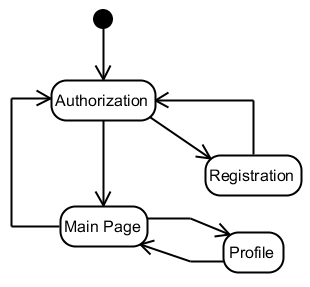
\includegraphics[width=0.8\textwidth]{screenFlow.png}
				\end{center}
			\end{column}
		\end{columns}
	\end{frame}

	\begin{frame}
		\frametitle{Wireframe}
		\begin{columns}
			\begin{column}{0.4\textwidth}
				\begin{itemize}
					\item Набор схематичных макетов
					\item Принципиально без дизайнерских подробностей, только положение элементов
					\item Используется как ТЗ, наглядный материал, первое приближение к дизайну
				\end{itemize}
			\end{column}
			\begin{column}{0.6\textwidth}
				\begin{center}
					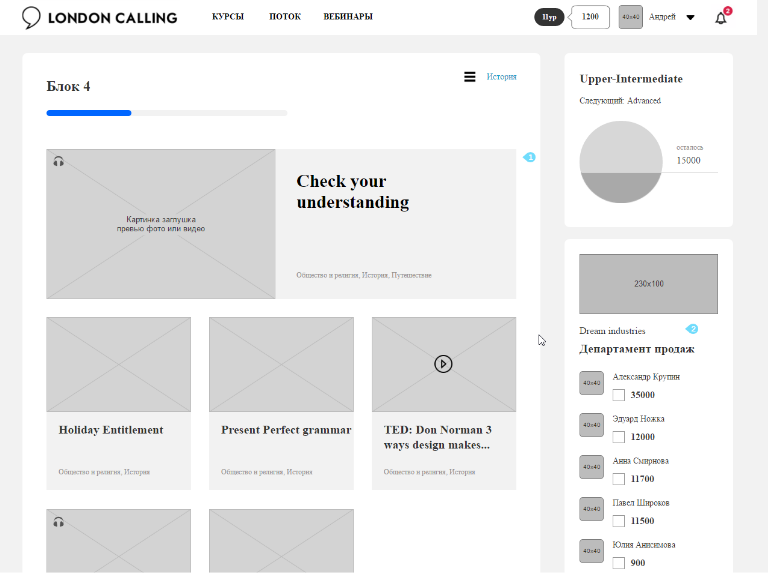
\includegraphics[width=\textwidth]{wireframe.png}
				\end{center}
			\end{column}
		\end{columns}
	\end{frame}

	\begin{frame}
		\frametitle{Дизайн-макет}
		\begin{columns}
			\begin{column}{0.4\textwidth}
				\begin{itemize}
					\item Разрабатывается дизайнером
					\item Похож на окончательный внешний вид интерфейса
					\item Часто с точностью до пиксела
				\end{itemize}
			\end{column}
			\begin{column}{0.6\textwidth}
				\begin{center}
					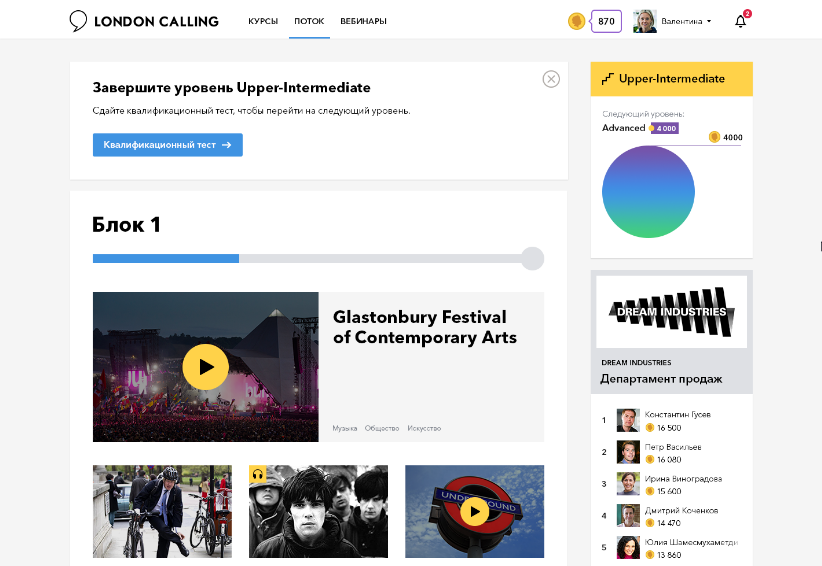
\includegraphics[width=\textwidth]{mockup.png}
				\end{center}
			\end{column}
		\end{columns}
	\end{frame}

	\begin{frame}
		\frametitle{Инструменты проектирования пользовательских интерфейсов}
		\begin{itemize}
			\item Balsamiq
			\begin{itemize}
				\item \url{https://balsamiq.com/products/mockups/}
				\item Кликабельные .pdf-ки
			\end{itemize}
			\item Ninjamock
			\begin{itemize}
				\item \url{https://ninjamock.com/}
				\item Бесплатный
				\item Веб-версия с коллаборацией
			\end{itemize}
			\item Axure
			\begin{itemize}
				\item \url{http://www.axure.com/}
				\item Продвинутый, но платный
			\end{itemize}
			\item UXPin
			\begin{itemize}
				\item \url{https://www.uxpin.com/}
				\item Продвинутый, но платный
				\item Зато браузерный
			\end{itemize}
		\end{itemize}
	\end{frame}

	\begin{frame}
		\frametitle{Ещё инструменты}
		\begin{itemize}
			\item Sketch
			\begin{itemize}
				\item \url{https://www.sketchapp.com/}
				\item Только под Mac
				\item Рисовалка интерфейсов, иконок и прочего
			\end{itemize}
			\item Figma
			\begin{itemize}
				\item \url{https://www.figma.com}
				\item Браузерный, коллаборативный
			\end{itemize}
			\item Invision app
			\begin{itemize}
				\item \url{https://www.invisionapp.com/}
				\item Браузерный, коллаборативный
				\item Кликабельные мокапы из картинок или Sketch-файлов
			\end{itemize}
		\end{itemize}
	\end{frame}

	\section{Задание}

	\begin{frame}
		\frametitle{Задача, UI}
		\framesubtitle{На пару и доделать дома}
		Спроектировать пользовательский интерфейс для своего проекта
		\begin{itemize} 
			\item Описать поток экранов в любом удобном виде
			\begin{itemize} 
				\item Диаграмма активностей
				\item Таблица
			\end{itemize} 
			\item Сделать набор макетов всех экранов приложения в каком-либо из инструментов создания wireframe-макетов 
		\end{itemize} 
		Результаты выложить на гитхаб и/или выложить на вики ссылку на проект в каком-либо из онлайн-тулов
	\end{frame}

\end{document}
